Otro de los trabajos que se realizó fueron algunas actividades con el sistema \textit{OBD} II y el \textit{CAN-BUS} de datos (\cite{GB1}), desarrollando la siguiente hipotesis. La solución que se propone es el desarrollo de una aplicación móvil mediante plataforma Android para poder modificar algunos parámetros y sensores del Sistema de Confort de un Vehículo de Gama media, utilizando de vehículo de pruebas un Stratus XLS 2006. \\

Las actividades que se desarrollaron fueron enfocadas a realizar pruebas en sistemas existentes en el mercado, estas se enlistan acotinuación:

\begin{itemize}
\item Funcionamiento del Can Bus y el conector DCL,
\item Funcionamiento del dispositivo EML327,
\item Funcionamiento de aplicaciones móviles,
\item Codificación y descodificación de la señal,
\item Pruebas y Resultados.
\end{itemize}

\paragraph{Funcionamiento del Can Bus y el conector DCL}
El desarrollo de esta actividad se llevó a cabo mediante la investigación de la metodología sobre el Sistema eléctrico del vehículo (\cite{GB1}), el can bus es el encargado de transmitir los códigos de falla del vehículo y el conector OBD, también conocido como conector de enlace de datos es el encargado pasar por medio de algún escáner los códigos al usuario, está ubicado normalmente en la parte inferior del volante.\\

Durante esta actividad también se realizaron pruebas con el osciloscopio, detectando los pines encargados de transmitir las señales por medio del CAN Bus, también denominados CAN \textit{High} y CAN \textit{Low}, los pines correspondientes son el número 2 y el 10, tal y como se muestra en la Figura \ref{Medos} debido a que cada marca maneja un protocolo ya establecido.

%
\begin{figure}[H]
%\vspace{0.2cm}
\centering
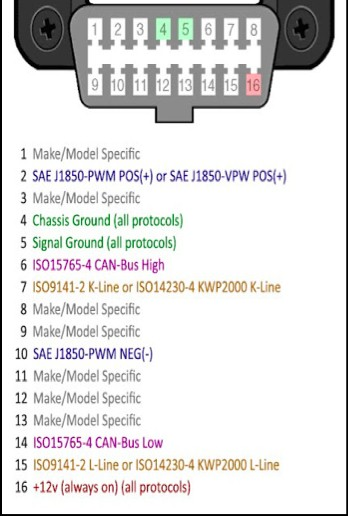
\includegraphics[width=0.3\textwidth]{metodologia/protocolos_obd.jpg}
\caption{Protocolos de comunicación con la configuración de los pines del conector DCL.}
\label{Medos}
\end{figure}
%

\paragraph{Funcionamiento del dispositivo EML327}

En la siguiente actividad se probaron algunas aplicaciones móviles existentes en el mercado para poder verificar por cuenta propia que el sistema Can Bus es capaz de enviar información relevante para el usuario a la hora de viajar en el vehículo (\cite{GB2}).\\

Por lo cual se realizaron pruebas con el escáner EML327, sin embargo este escáner funciona únicamente  para el sistema de tracción, esto permitió realizar las primeras pruebas en el vehículo sobre el escaneo de información a una aplicación móvil mediante tecnología Bluetooth. \\

Primeramente se conectó el EML327 al conector de enlace de datos tal cual se muestra en la Figura \ref{Metres}\\

%
\begin{figure}[H]
%\vspace{0.2cm}
\centering
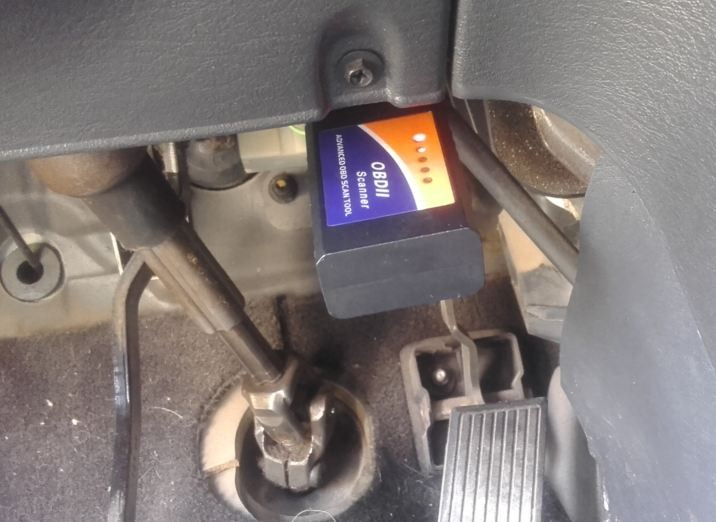
\includegraphics[width=0.5\textwidth]{metodologia/elm327.jpg}
\caption{dispositivo EML 327 conectado al vehículo.}
\label{Metres}
\end{figure}


\paragraph{Funcionamiento de aplicaciones móviles}

Después se buscó en la tienda de Google Play aplicaciones compatibles con el escáner EML327, se obtuvieron dos aplicaciones``Scanner OBD" y ``Piston”, se descargaron y se procedió a visualizar el funcionamiento de ambas. La aplicación Escáner OBD muestra información sobre el protocolo de comunicación la cual se muestran en las Figuras \ref{Mecuatro}. 

\begin{figure}[H]
\centering
\subfigure[]{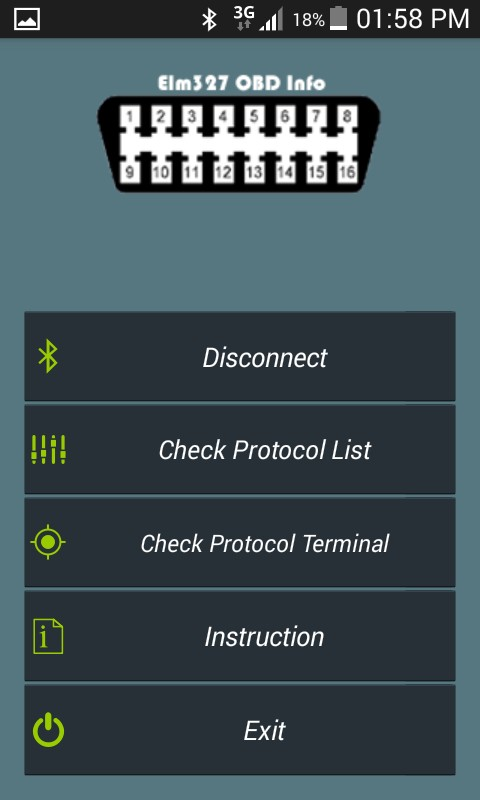
\includegraphics[width=60mm]{metodologia/eml327.jpg}}\hspace{10mm}
\subfigure[]{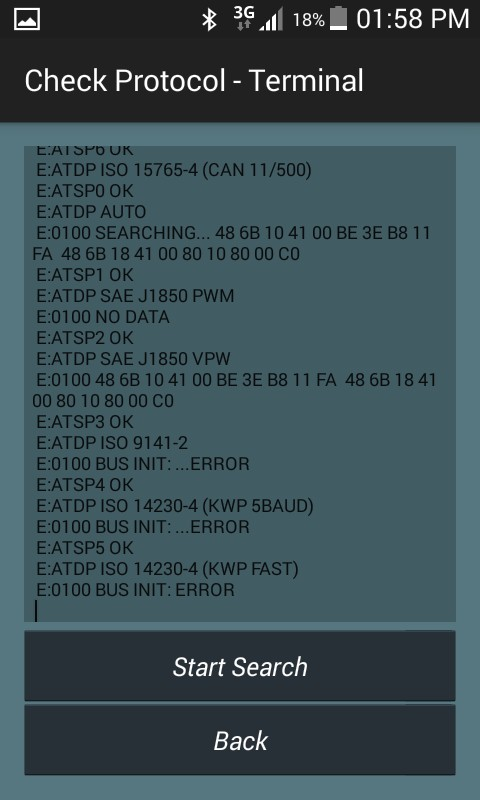
\includegraphics[width=60mm]{metodologia/eml327_.jpg}}
\caption{Pantallazos de la aplicación Scanner OBD.} \label{Mecuatro}
\end{figure}


La aplicación “Piston” muestra información sobre el sistema de tracción como el voltaje de la batería, la temperatura del agua, las revoluciones por minuto y la velocidad, tal cual se muestra en la Figura \ref{Mecinco}.

\begin{figure}[H]
\centering
{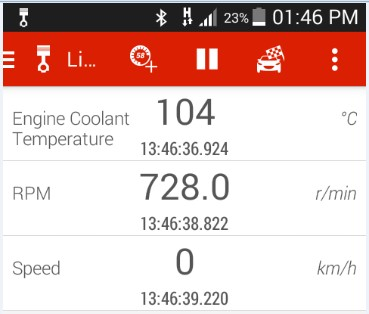
\includegraphics[width=0.6\textwidth]{metodologia/piston.jpg}}
\caption{Pantallazo de la aplicación Piston.} \label{Mecinco}
\end{figure}



\paragraph{Codificación y descodificación de la señal}

Para esta actividad, se vio en la necesidad de conocer completamente el sistema de confort, principalmente en la parte del sistema eléctrico. \\

Por protocolos de seguridad las armadoras no permiten el acceso al mismo, sin embargo algunas asociaciones de mecánicos en el país tienen acceso a ellos mediante software que los auxilia a reparar los vehículo, como es el caso del software OnDemand5 (\cite{GB3}).\\
